%here we wish to summarize everything related to "adaptive Gaussian filters"
%in one .tex file
%we take as much as we can directly from the master's thesis...

%\pagestyle{myheadings}

\documentclass[11pt]{article}

\usepackage{amsmath}
\usepackage[dvips]{graphicx}
%\bibliographystyle{elsart-harv}
\usepackage{url}

\bibliographystyle{plain}


\begin{document}

\begin{center}

{\LARGE Adaptive Gaussian filters: a powerful new method for supervised learning}
\vspace{5mm}

{\large Peter Mills\footnote
{Correspondence should be sent to: \newline
Peter Mills \newline
(peteymills@hotmail.com) \newline
49-421-218-7045 (phone) \newline
49-421-218-4555 (fax)}\newline
}
\textit{
Institute for Environmental Physics, \newline
University of Bremen, \newline
PO Box 330440, \newline
28334 Bremen, \newline
Germany}\newline

\end{center}

\begin{flushleft}

\section*{Abstract}
Adaptive Gaussian filtering (AGF) is a new method for estimating
probability densities and performing statistical classification.
Its justification is a generalization of a $k$-nearest-neighbours
whereby the training samples are weighted by distance
using a symmetric filter function and the total of the weights 
is constrained to a constant value by varying the width of the
filter.  A Gaussian is chosen 
because of its mathematical properties--it is easy to solve
for the filter width, for instance.  
Probability estimates 
can be used directly or they can be used to search for a 
class border from which estimates of both the
class and the conditional probabilities are easy to extrapolate.
The method is validated on a pair of two-dimensional synthetic
test classes and compared
to three of the most popular existing methods.  
As applied to the test case it is shown
to be over twenty-five (25) times as fast as the equivalent
analysis using a support vector machine (SVM), with no loss of
accuracy, while being easier to apply and understand.

\vspace{3mm}

\emph{Keywords:}\newline
Monte Carlo methods \newline
statistical classification \newline
supervised learning \newline
PDF estimation

\pagebreak

%\input{agf_symbols.tex}

\tableofcontents

\parindent=5mm
\newcommand{\filtfunc} f

\section{Introduction}

Statistical classification is one of the most commonly employed
forms of machine learning.  It is useful both for its own sake--to
classify a test point based on known inputs--and for non-linear
regression by dividing a continuum variable into discrete
ranges.

This paper discusses a new and very simple method of statistical
classification, validates it on a pair of synthetic test classes
and compares it with three other popular methods.

\section{Adaptive Gaussian filtering}
\label{AGF_intro}

The $k$-nearest neighbours (KNN) is a well-known and effective technique of
estimating probability densities and performing classifications.
A simple refinement to this method would be to weight the samples
according to distance, much like in a simple linear filter.
Given a set of points, $\lbrace \vec x_i\rbrace$, 
the probability density function (PDF)
for a test point $\vec x$ may be estimated as follows:
\begin{eqnarray}
P(\vec x) & \approx & \frac{W}{n N} \label{pdf_est} \\
W & = & \sum_{i=0}^n w_i
\label{W_def}
\end{eqnarray}
where $w_i$ is the weight of the $i$th sample, $n$ is the number
of samples and $N$ is a normalisation coefficient.  Its justification
is a Monte Carlo integration with importance sampling, except that
here we solve for the importance distribution by multiplying it
with a peaked, but otherwise essentially arbitrary function, and
assume that it is roughly constant.

The magnitude
of the weights must decrease with distance and in the isotropic
case they are given by:
\begin{eqnarray}
w_i & = & \filtfunc(d_i) \\
d_i & = & | \vec x - \vec x_i |
\end{eqnarray}
where $\filtfunc$ is a filtering function and $d_i$ is the 
distance of the $i$th
sample from the test point.  The upright brackets denote a metric,
typically Cartesian, although in theory any metric could be used.
In practice, it is often simplest and most efficient to first re-
scale or otherwise transform the variables so that a Cartesian metric
is then appropriate.  The normalisation coefficient will be given by:
\begin{equation}
N =  \int_A \filtfunc(|\vec x - \vec y|) dy
\end{equation}
where $A$ is the domain of the samples.

A natural choice for $\filtfunc$ would be a Gaussian:
\begin{equation}
\filtfunc(r) = \exp \left (- \frac{r^2}{2 \sigma^2} \right )
\label{Gaussian_filter}
\end{equation}
where $\sigma$ is the filter width and $N = (2 \pi)^{D/2} \sigma^D$
with $D$ as the number of dimensions.  Using a fixed filter width
may mean that in regions of low density, all samples will fall in
the tails of the filter with very low weighting, while regions of
high density will find an excessive number of samples in the central
region with weighting close to unity.  Thus we vary the
filter width according to density so that an optimal number of
samples fall within the central region.

According to the definition of the probability density, the local
average point spacing will be given as follows:
\begin{equation}
\delta = \frac{1}{\left [ n P(\vec x) \right ]^{1/D}}
\end{equation}
We wish to vary the filter width so that it matches the point spacing:
\begin{equation}
\sigma^{(opt)} = k_1 \delta = \frac{k_1}{\left [ n P(\vec x) \right ]^{1/D}}
\end{equation}
where $k_1$ is a coefficient.
Substituting the approximated PDF from (\ref{pdf_est}) through
(\ref{Gaussian_filter}) produces the
following that must be solved for $\sigma^{(opt)}$:
\begin{equation}
W (\sigma^{(opt)}) \approx k_1^D (2 \pi)^{D/2}
\label{opt_filt2}
\end{equation}
Thus, correctly selecting a fixed value for $W$ (call it $W_c$) in
(\ref{W_def}) should produce an ``optimal'' (as we have defined it)
filter width. 
The quantity $W_c$ may be thought of as roughly equivalent to $k$ in a
$k$-nearest neighbours scheme.

\section{Solving for the filter width}

The properties of the exponential function can be used to 
solve for the filter width by iteratively squaring the weights.  Let the $j$th
weighting coefficient of the $i$th sample be given as:
\begin{equation}
w_i^{(j)} = \exp \left ( \frac{d_i^2}{2 ( \sigma^{(j)})^2} \right )
\end{equation}
where $\sigma^{(j)}$ is the $j$th filter width.  Each subsequent iterate is
defined as the square of its previous:
\begin{equation}
w_i^{(j)} = \left (w_i^{(j-1)} \right )^2
\end{equation}
consequently the jth filter width, $\sigma^{(j)}$, obeys the following
recursion relation:
\begin{equation}
\sigma^{(j)} = \frac{\sigma^{(j-1)}}{\sqrt{2}}
\end{equation}
Following our super-scripting convention, $W^{(j)}$ is defined as:
$W^{(j)} = \sum_i w_i^{(j)}$ with the final iteration of $j$, call it
$f$, defined such that:
\begin{equation}
W^{(f)} \le W_c
\end{equation}
Obviously, the initial filter width, $\sigma^{(0)}$, must be chosen to be larger
than the optimal, for instance by taking the total variance of the data.

The final filter width is approximated by exponential interpolation to
the target total weight:
\begin{eqnarray}
k_2 & = & \frac{\log W_c + \log W^{(f)} - 2 \log W^{(f-1)}}{2\left
	(\log W^{(f)} - \log W^{(f-1)}\right )} \\
\sigma^{(opt)} & \approx & \frac{\sigma^{(f)}}{\sqrt{k_2}}
\end{eqnarray}
To use the method for classifications, the
conditional probability is estimated as follows:
\begin{equation}
P(m | \vec x) \approx \frac{1}{W} \sum_{i, c_i=m} w_i
\end{equation}
where $c_i$ is the class associated with the $i$th sample.
The class of which $\vec{x}$ is most likely a member
will be given by the value of $j$ supplying the maximum value of this PDF:
\begin{equation}
c=\arg \underset {j} {\max} P(j | \vec{x})
\label{class_mle}
\end{equation}

\section{Finding the class borders}

The chief advantage of this scheme over a $k$-nearest neighbours is that
it produces results that are both continuous and differentiable.  
Both properties are desirable in that they allow us to search for a unique
border between the classes and hence make more rapid classifications. 
Assuming that there are
only two classes, the difference in their conditional probabilities is:
\begin{equation}
R(\vec x) = P(2 | \vec x) - P(1 | \vec x) \approx \frac{1}{W}
\sum_i (2 c_i - 3) w_i
\label{Rdef}
\end{equation}
where $1$ and $2$ are the classes and $c_i$ is the class of the $i$th sample.
The borders are found by setting this expression to zero,
$R(\vec x)=0$.  With an adaptive Gaussian filter, the derivative becomes:
\begin{equation}
\frac{\partial R}{\partial x_j} \approx \frac{1}{W_c (\sigma^{(opt)})^2}
	\sum_i w_i^{(opt)} (2 c_i - 3) \left [x_{ij}-x_j - d_i^2 \frac{\sum_k
	w_k^{(opt)} (x_{kj}-x_k)} {\sum_k d_k^2 w_k^{(opt)}} \right ] 
\label{class_grad}
\end{equation}
where $x_{ij}$ is the $j$th coordinate of the $i$th sample, while $x_j$ is the
$j$th coordinate of the test point.

The procedure employed (although others are possible)
 is as follows:  pick two points at random,
$\vec x_1$ and $\vec x_2$, belonging to classes 1 and 2 respectively.  We
define $\vec v$ as a direction vector between the two points, e.g.:
\begin{equation}
\vec v = \vec x_2 - \vec x_1
\end{equation}
and solve the following for t:
\begin{equation}
R(\vec x_1 + \vec v t) = 0
\end{equation}
to find a point,  $\vec b = \vec x_1 + \vec v t|_{R=0}$, 
randomly located on the class border.
The derivatives, $dR/dt = \nabla_{\vec x} R \cdot \vec v$, are used
 as an aid to root-finding
by fitting a third-order polynomial and using this
to estimate the root.  The true root is then rebracketed with this new estimate, 
combining fast convergence with numerical stability.
The GNU scientific library (GSL) is used both to 
solve the cubic and to fit the function by
solving the rank four linear system using Householder
transformations. \cite{gsl_ref}
\linebreak
\linebreak
The border may be thus sampled as many times as necessary,
giving a set of vectors, $\lbrace \vec b_i \rbrace$, 
along with their corresponding gradients,
$\lbrace \nabla_{\vec x} R (\vec b_i) \rbrace$.  The class of a test point,
$\vec x$, is calculated as follows:
\begin{eqnarray}
j & = & \arg \underset{i}{\min} | \vec b_i - \vec x | \label{jeq}\\
p & = & (\vec x - \vec b_j) \cdot \nabla_{\vec x} R (\vec b_j) \label{peq} \\
c & = & ( 3 + p/|p| ) / 2 \label{ceq}
\end{eqnarray}
where $c$ is the class.  

\section{Extrapolating the conditional probabilities}

The value of $R$ may be extrapolated to the test point.
Consider a pair of one dimensional classes composed of two equal-sized 
Gaussians of width $s$ separated by a distance $2a$ 
with the class border lying at $b$.
Let $\tilde R$ be the difference between the conditional probabilities:
\begin{eqnarray}
  \tilde R(x) & = & P(2|x) - P(1|x) \\
  & = & \frac{P(2, x) - P(1, x)}{P(1, x) + P(2, x)} \\
  & = & \frac{e^{-\frac{(x-b+a)^2}{2 s^2}} -
                e^{-\frac{(x-b-a)^2}{2 s^2}}}
                {e^{-\frac{(x-b+a)^2}{2 s^2}} +
                e^{-\frac{(x-b-a)^2}{2 s^2}}}
\end{eqnarray}
Simplifying:
\begin{equation}
\tilde R (x) = \tanh \left (\frac {a(x-b)}{s^2} \right )
\label{cext:r1sim}
\end{equation}
To approximate the difference in
conditional probabilities, $R(x)$, between an arbitrary pair of (well-behaved)
1-D classes, we fit the function by setting:
\begin{eqnarray}
\tilde R(b) = R(b) & = & 0 \\
\frac{d\tilde R(b)}{dx} = \frac{a}{s^2} & = & \frac{dR(b)}{dx}
\end{eqnarray}
We can approximate R for a pair of multi-dimensional classes 
in the same way:
\begin{equation}
R(\vec x) \approx \tilde R(\vec x) \equiv \tanh p
\label{confidence_est}
\end{equation}
It is easy to show:
\begin{eqnarray}
\tilde R(\vec b_j) & = & 0 \\
\nabla_{\vec x} \tilde R(\vec b_j) & = &\nabla_{\vec x} R(\vec b_j)
\end{eqnarray}

\section{A pair of test classes}
\label{test_classes}

\begin{figure}
\resizebox{1\textwidth}{!}{
  \includegraphics{sample_class_bw.ps}}
%  \includegraphics[width=1\textwidth]{sample_class_bw.ps}%}
  \caption{A pair of synthetic test classes}
  \label{cls_exmpl}
\end{figure}

The AGF method was tested on a synthetic dataset consisting of the pair of
classes shown in figure \ref{cls_exmpl}.  The first class, illustrated using
triangles, is a simple, two-dimensional normal distribution:
\begin{eqnarray} 
P(\vec x | 1) & = & \frac{1}{2 \pi \sigma_1 \sigma_2} 
	\exp \left \lbrace - \frac{1}{2}\left 
	[\left (\frac{x^\prime}{\sigma_1}\right )^2 + 
	\left (\frac{y^\prime}{\sigma_2} \right )^2 \right ] \right \rbrace
\label{pdf_sc1a} \\
\vec x^\prime & = & \left [\begin{array}{cc} 
	\cos \theta & \sin \theta \\
	-\sin \theta & \cos \theta
\end{array} \right ] \cdot (\vec x - \vec x_0) 
\label{pdf_sc1b} 
\end{eqnarray}
where $\vec x_0$ is the centre of the distribution, $\sigma_1$ and $\sigma_2$ are
the widths of its major and minor axes respectively, $\theta$ is the 
angle of the major axis and $\vec x^\prime = (x^\prime, y^\prime)$.

To produce a non-trivial interface between the two classes, 
the second one has a more intricate design.
A set of points defining the ``backbone'' of the distribution was chosen.
Individual samples are first interpolated a random distance along 
the curve so defined using a cubic spline. \cite{nr_inc2} \cite{gsl_ref}
By displacing this point a random distance in a random direction, 
the final location of the sample is determined.

Analytic or semi-analytic values for the probability densities of
the second class may be calculated as follows:
\begin{equation}
P(\vec x | 2) = \frac{1}{s_{max}}\int_0^{s_{max}} Q(|\vec x - \vec g(s)|) ds
\label{pdf_sc2}
\end{equation}
where $\vec g$ is the line segment
defining the ``backbone'', $s$ is the path along it, $s_{max}$ is its
length and $Q(r)$ is a circularly symmetric
PDF governing the offset distance from the backbone.
For the dataset shown in figure \ref{cls_exmpl}, a Gaussian was once 
again employed for $Q$.

\section{Validating the probability density functions}

\begin{figure}
  \resizebox{0.9\textwidth}{!}{%
    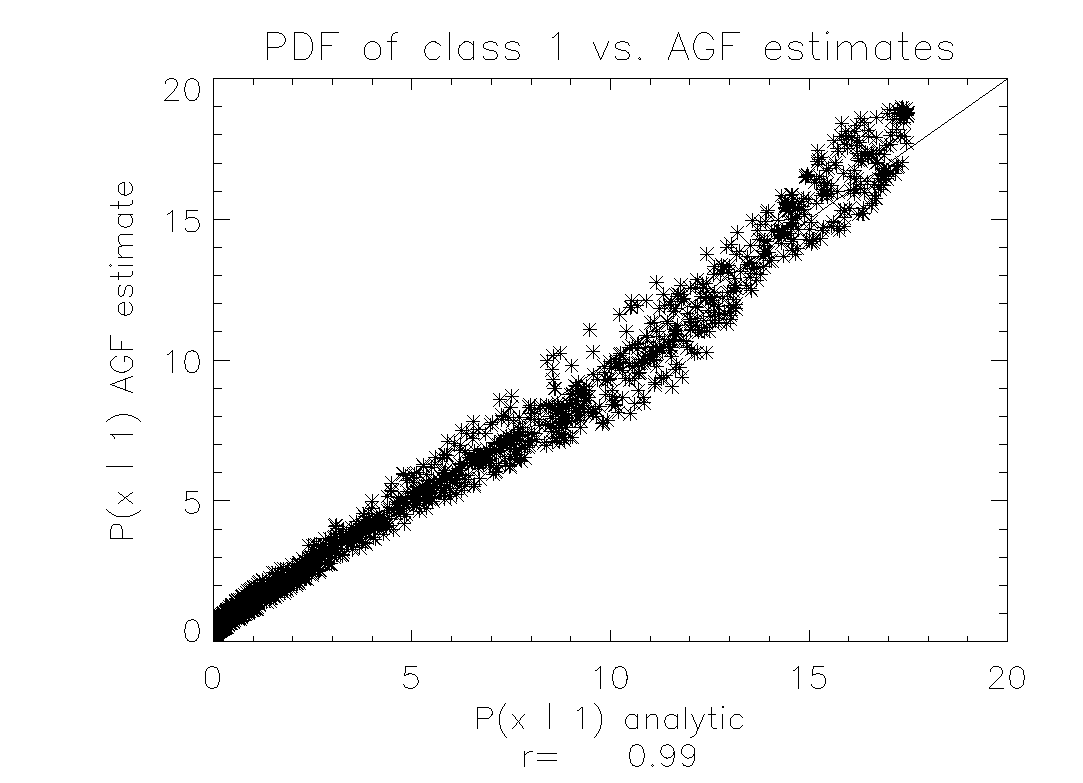
\includegraphics{pdf1_agf.eps}}
%  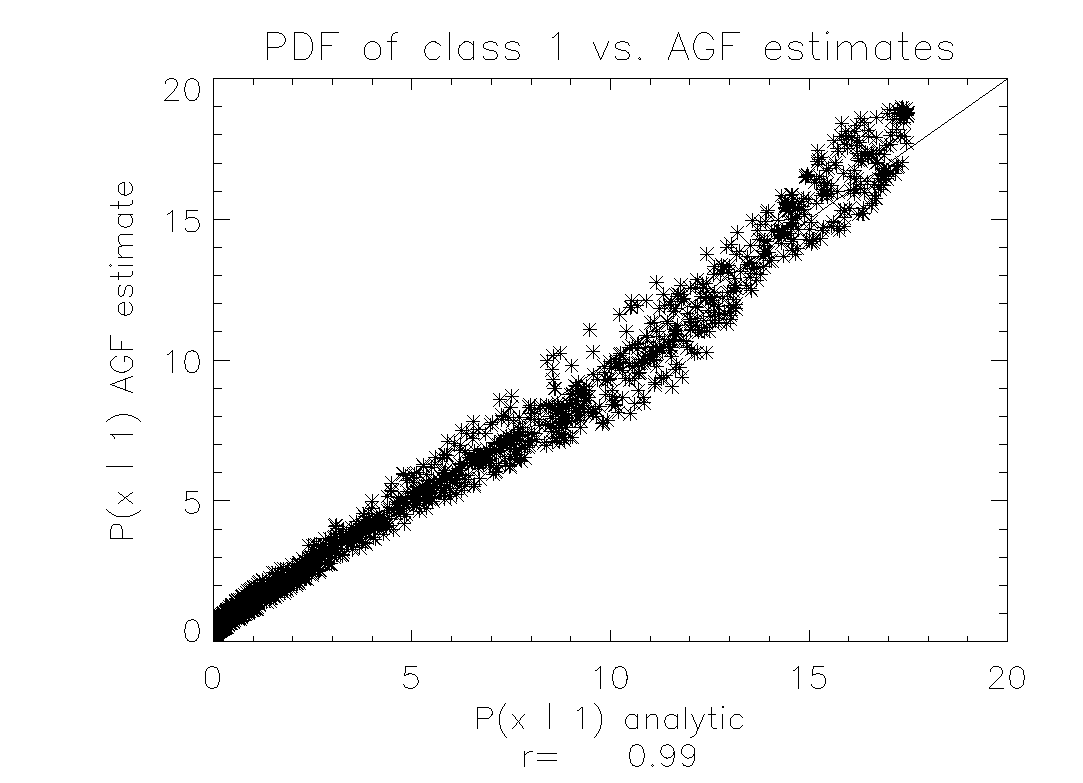
\includegraphics[width=0.9\textwidth]{pdf1_agf.eps}
  \label{pdf1_agf}
  \caption{A comparison of PDF estimates with calculated analytic values}
\end{figure}

\begin{figure}
  \resizebox{0.9\textwidth}{!}{
    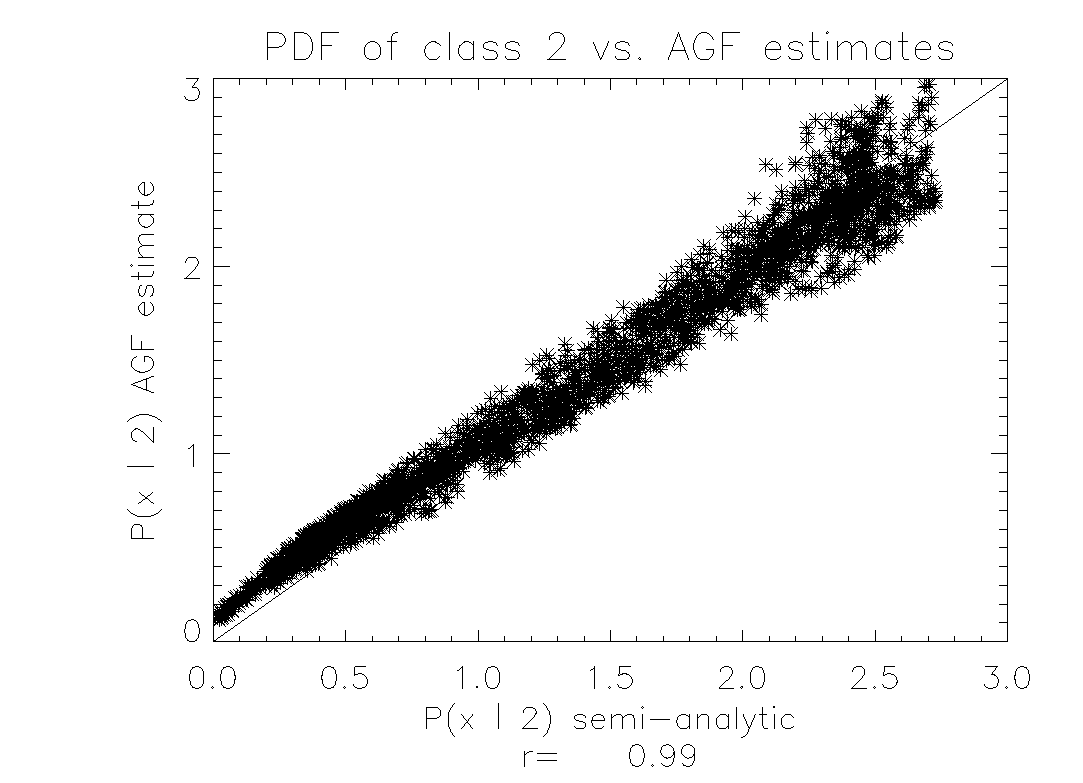
\includegraphics{pdf2_agf.eps}}
%  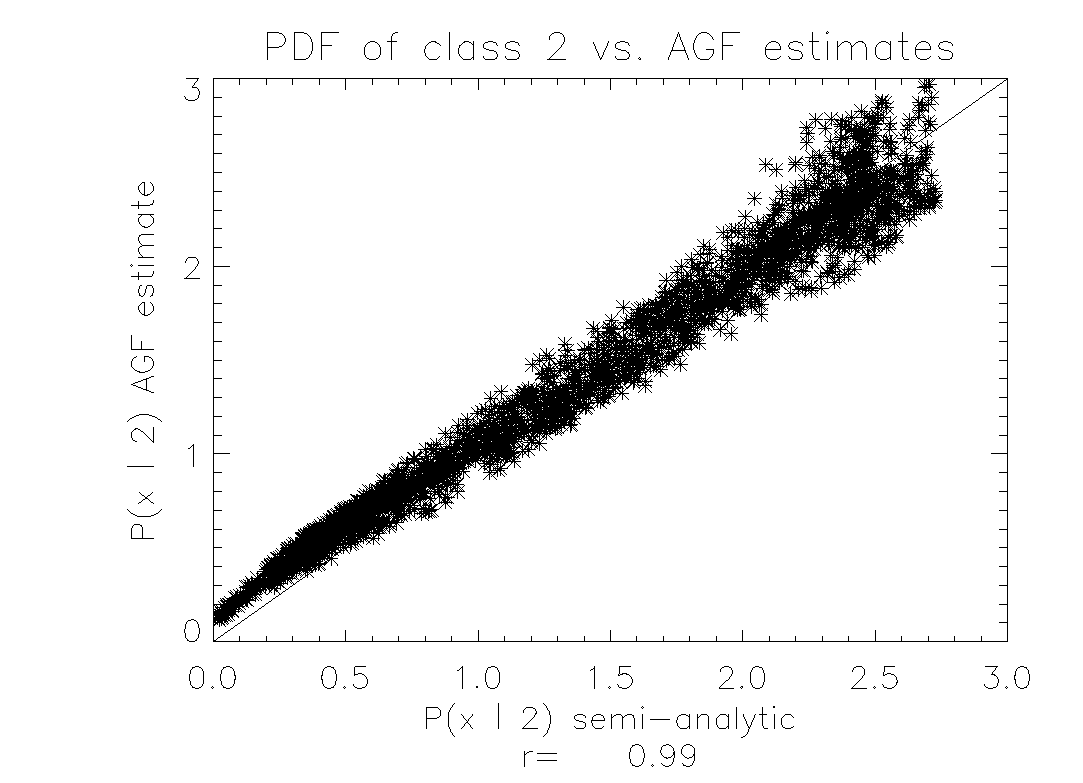
\includegraphics[width=0.9\textwidth]{pdf2_agf.eps}
  \caption{A comparison of PDF estimates with calculated, semi-analytic values}
  \label{pdf2_agf}
\end{figure}

Random synthetic datasets composed of 5000 samples of the first class
and 10000 samples of the second class were created as needed
using the algorithms described in section \ref{test_classes}.
Test datasets composed of three-thousand (3000) members
were created separately and had no fixed ratio
between the number of members in each class.  Rather the
ratio of the training data was used to randomly select which
class was sampled.

The PDFs estimated from equation (\ref{pdf_est}) may 
be compared to analytical and semi-analytical values calculated
from equations (\ref{pdf_sc1a}) and (\ref{pdf_sc2}).
Of course, statistical estimates will be slow because there
is no training phase--each estimate relies on the entire store
of training data.

PDF estimates for both classes are shown in figures \ref{pdf1_agf}
and \ref{pdf2_agf}.  To calculate reference values for the second
class, equation (\ref{pdf_sc2}) was integrated numerically by
summing one-thousand (1000) samples using a mid-point method.
The critical weight, $W_c$, chosen was one-hundred (100) for both
classes.
We would expect errors
of density estimates to scale with the density itself, 
as seen in the plots, although there is a considerable bias for
the very lowest densities, especially for the second class.

\section{Comparison with other methods}

To test the viability of this new classification algorithm,
it was compared with three other, popular methods.
These are: $k$-nearest-neighbours (KNN), learning vector quantization (LVQ)
and support vector machines (SVM) and are briefly described
below.

\subsection{K-nearest-neighbours}

The $k$-nearest neighbours is one of the simplest and most robust
classification methods available.  It consists of finding the
the $k$ training samples that are closest to the test point and then
counting how many there are of each class.  The class with the most
samples is the class of the test point.

Our method reduces to a KNN by using a filter function that
is one out to the filter width and zero everywhere else:
\begin{equation}
\filtfunc(r) = \left \lbrace \begin{array}{lr}
\filtfunc(r) = 1 , & r < \sigma \\
\filtfunc(r) = 0 , & r \ge \sigma
\end{array} \right .
\end{equation}
where $\sigma$ is the filter width.

\subsection{Learning vector quantization}

Learning vector quantization works by building up a set of ``codebook vectors''
whose density matches the difference between the densities of the
two classes.  The vectors will be labelled based on which class they
fall within.  The class of a test point will be given by the class
label of the nearest codebook vector.

The training process is performed as follows:  a set of codebook
vectors are initialized at random points and assigned class labels.  
The codebook vectors are randomly compared with the training samples.
If the labels of the two match, then the codebook vector is moved
closer to the training sample.  If they don't, then it is moved farther
away.  \cite{Kohonen2000} \cite{LVQ_PAK}

\subsection{Support vector machines}

In support vector machines, a single hyperplane is drawn that best
divides the two classes.  Classifications are done as in equations
(\ref{jeq}) through (\ref{ceq}) based on a dot product with the normal
to the class border.  The border is fitted by minimizing the classification
error.  Obviously, using a single straight line to divide the two
synthetic sample classes will produce poor results. 
Results may be improved by 
adding variables derived from
the originals thus expanding the dimension of the space, 
much as one fits a set of basis functions by performing a linear
fit on the set of variables formed by transforming the independent variables
with the basis functions.

The so-called kernel trick can be applied to most algorithms
that use scalar products and is based on the observation that certain
mathematical operations applied to a scalar product will expand the
dimensionality of the space, without having to add extra variables.
For example, consider the squared dot product of two two-dimensional 
variables: \cite{Mueller_etal2001}
\begin{eqnarray}
(\vec x \cdot \vec y)^2 & = & [(x_1, x_2) \cdot (y_1, y_2)]^2 \\
& = & x_1^2 x_2^2 + 2 x_1 y_1 x_2 y_2 + x_2^2 y_2^2 \\
& = & (x_1^2, \sqrt{2} x_1 x_2, x_2^2) \cdot (y_1^2, \sqrt{2} y_1 y_2, y_2^2)
\end{eqnarray}
The algorithm was also compared with an analytical classification
scheme that compares the results of equations (\ref{pdf_sc1a}) and 
(\ref{pdf_sc2}) applied to the test point.  This has the advantage
of quantifying the limit in accuracy of any classification algorithm,
as well as returning the conditional probabilities.

\begin{table}
  \begin{center}
  \caption{Comparison of parameters used in the KNN, LVQ, AGF
	and AGF borders classification algorithms}
  \begin{tabular}[h]{|l|l|l|l|}\hline
    KNN & LVQ & AGF & AGF borders \\ \hline \hline
    $k = 51$ & $\alpha_0=0.1$ & $W_c = 100$ & $W_c=100$ \\
      & $n_t=75000$ & $k=1000$ & $k=1000$ \\
      & $n=1000$ & & $n=250$ \\ 
      & & & $\epsilon=0.0001$ \\ \hline
  \end{tabular}
  \label{parm_table}
  \end{center}
\end{table}

\begin{table}
  \begin{center}
  \caption{Parameters used in the SVM classification algorithm}
  \begin{tabular}[h]{|ll|}\hline
    implementation: & LIBSVM \\
    type: & C-SVC \\
    kernel basis function: & $\exp(\gamma |\vec x_i - \vec x_j|^2)$ \\
    $\gamma$: & $0.5$ \\
    $C$ (cost): & $100$ \\ 
    $\epsilon$: & $0.001$ \\ \hline
  \end{tabular}
  \label{SVM_parm}
  \end{center}
\end{table}
    
Parameters for the KNN, LVQ, AGF and AGF borders technique are
compared in table \ref{parm_table}.  For the LVQ method, Kohonen's
so-called optimized LVQ 1 (OLVQ1) method was used.  $n_t$ is the 
number of training cycles, while $n$ is the number of codebook
vectors for the LVQ method and the number of border samples for
the AGF border classification method.  Note that AGF can be applied
directly without searching for the class borders.  
Also, performing the AGF classifications with all the data would
be too slow, so the $k$-nearest-neighbours supplying the most 
weight are selected before
applying the algorithm.  This is done in $n \log k$ time using a
binary tree.  The parameters used for the SVM method are listed
in table \ref{SVM_parm}.  The parameter, $\epsilon$, represents
the fitting tolerance for both AGF and SVM.

\section{Results}

\begin{table}
  \begin{center}
  \caption{Summary of validation and comparison results}
     \begin{tabular}{|l|c|c|c|c|c|} \hline
       Algorithm &     training &  classification & uncertainty &      accuracy &   correlation \\
                 &     time (s) &  time (s)       & coefficient &               & of R \\ \hline\hline
        Analytic &     N/A &  $1.29 \pm 0.20$ & $0.53 \pm 0.02$ & $0.906 \pm 0.005$ & $1.$ \\ \hline
             KNN &     N/A &  $5.59 \pm 0.31$ & $0.53 \pm 0.02$ & $0.905 \pm 0.005$ & $0.9953 \pm 0.0006$\\ \hline
             AGF &     N/A &  $9.40 \pm 0.31$ & $0.53 \pm 0.02$ & $0.905 \pm 0.005$ & $0.9979 \pm 0.0003$\\ \hline
     AGF borders & $4.19\pm0.10$ & $0.013\pm0.002$ & $0.53\pm0.02$ & $0.905\pm0.005$ & $0.9972 \pm 0.0008$\\ \hline
             LVQ & $2.81\pm0.01$ & $0.101\pm0.003$ & $0.50\pm0.02$ & $0.898\pm0.006$ &  N/A \\ \hline
             SVM & $112.4\pm3.6$ & $2.22\pm0.15$ & $0.53\pm0.02$ & $0.905\pm0.005$ & $0.9978\pm 0.0003$ \\ \hline
    \end{tabular}
    \label{comp_table}
  \end{center}
\end{table}

Table \ref{comp_table} shows the results of the comparison over twenty (20)
trials.  The uncertainty
coefficient is a better method of validating classification results
than simple accuracy (fraction of correct guesses) and is defined as follows:
\begin{eqnarray}
  H(i|j) & = & - \sum_{i, j} P(i, j) \ln P(i|j)\\
  H(i) & = & \sum_i P(i) \ln P(i) \\
  U(i|j) & = & \frac{H(i)-H(i|j)}{H(i)}
\end{eqnarray}
where $i$ and $j$ enumerate the true and retrieved classes respectively, 
$P(i, j)$ is their joint probability, $P(i|j) = P(i, j)/P(j)$ is their
conditional probability, and $P(i) = \sum_j P(i, j)$ is the total,
invariant probability of the first class.  If we think of the classification
procedure as a noisy channel, then $U(i|j)$ quantifies how many bits of knowledge
we have of the true value of the class as a fraction of the maximum
number of bits it is possible to transmit per classification.
\cite{nr_inc2} \cite{Shannon}

The last column in the table is simply the correlation coefficient of the
estimates of $R(\vec x)$ vs. the true values as computed by equations
(\ref{pdf_sc1a}) through (\ref{pdf_sc2}).  For a visual comparison, see figures
\ref{con_knn} through \ref{con_svm}.  Figure \ref{con_agf2} compares
estimates from AGF with borders training and without.

\begin{figure}
  \resizebox{0.9\textwidth}{!}{
    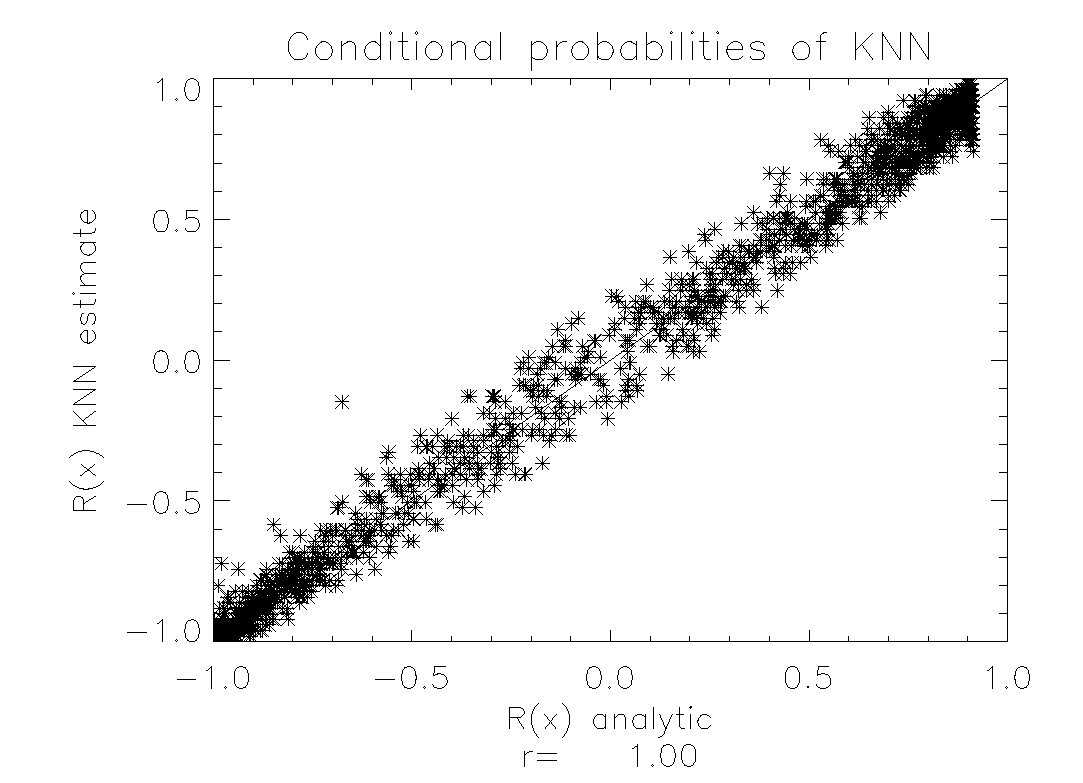
\includegraphics{con_knn.eps}}
%  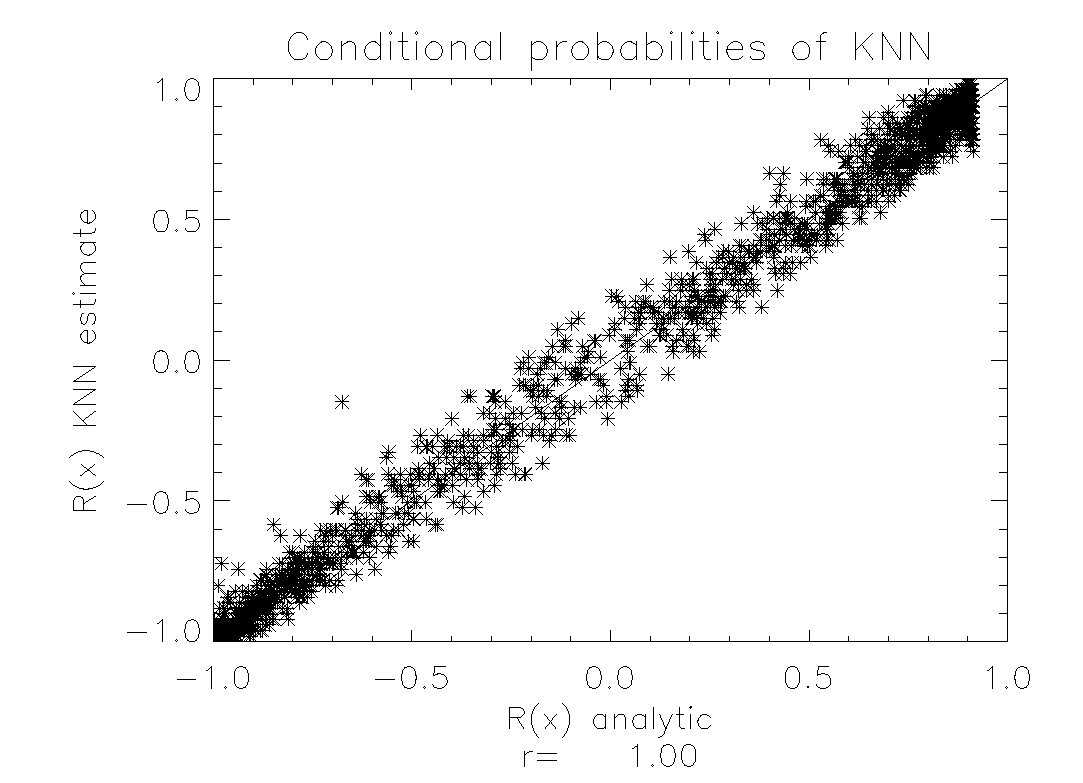
\includegraphics[width=0.9\textwidth]{con_knn.eps}
  \caption{Estimates of conditional probabilities.}
  \label{con_knn}
\end{figure}

\begin{figure}
  \resizebox{0.9\textwidth}{!}{
    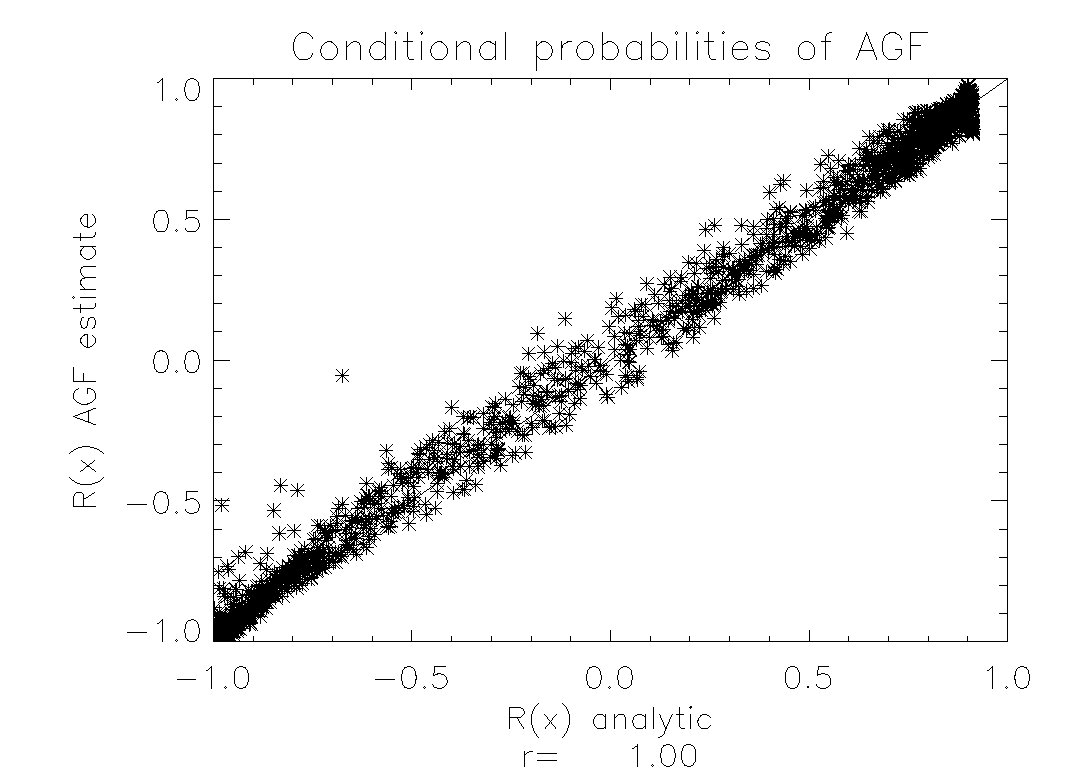
\includegraphics{con_agf.eps}}
%  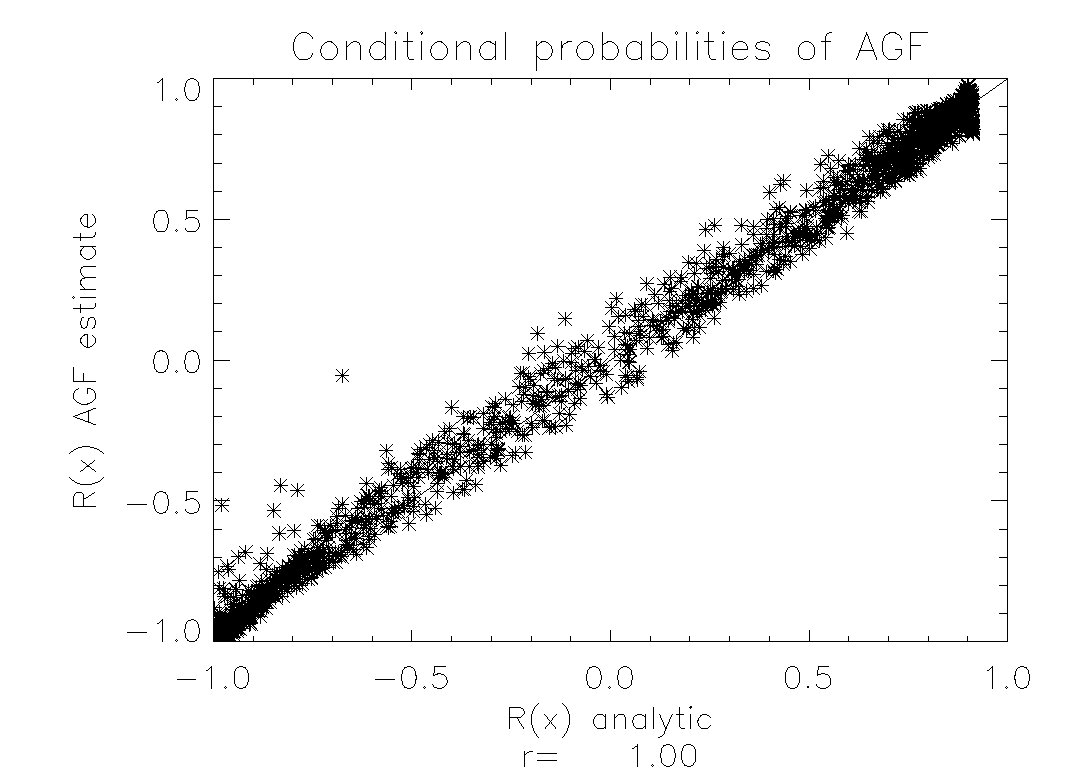
\includegraphics[width=0.9\textwidth]{con_agf.eps}
  \caption{Estimates of conditional probabilities.}
  \label{con_agf}
\end{figure}

\begin{figure}
  \resizebox{0.9\textwidth}{!}{
    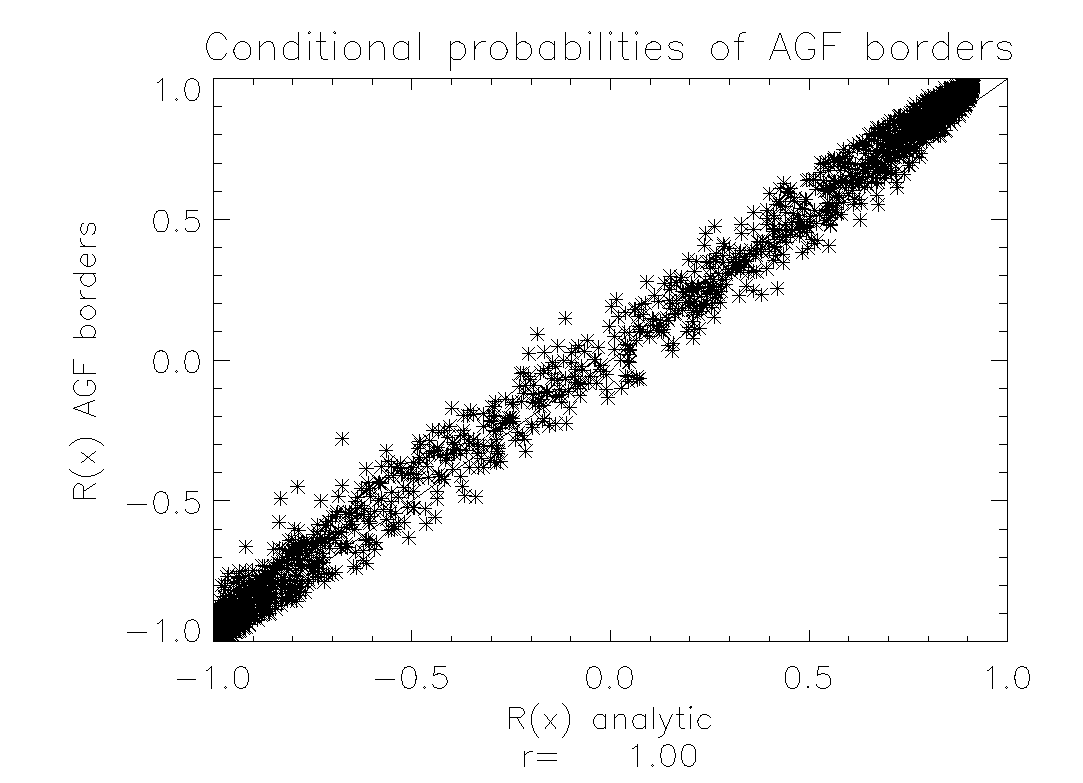
\includegraphics{con_agf_bord.eps}}
%  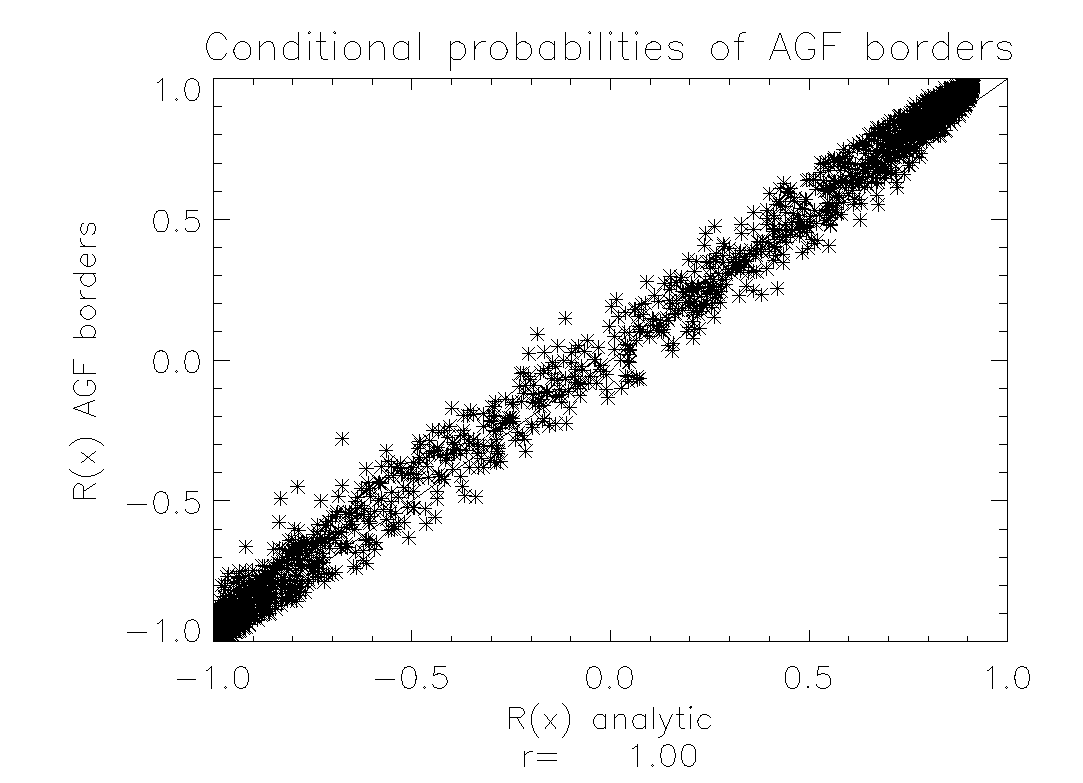
\includegraphics[width=0.9\textwidth]{con_agf_bord.eps}
  \caption{Estimates of conditional probabilities.}
  \label{con_agf_bord}
\end{figure}

\begin{figure}
  \resizebox{0.9\textwidth}{!}{
    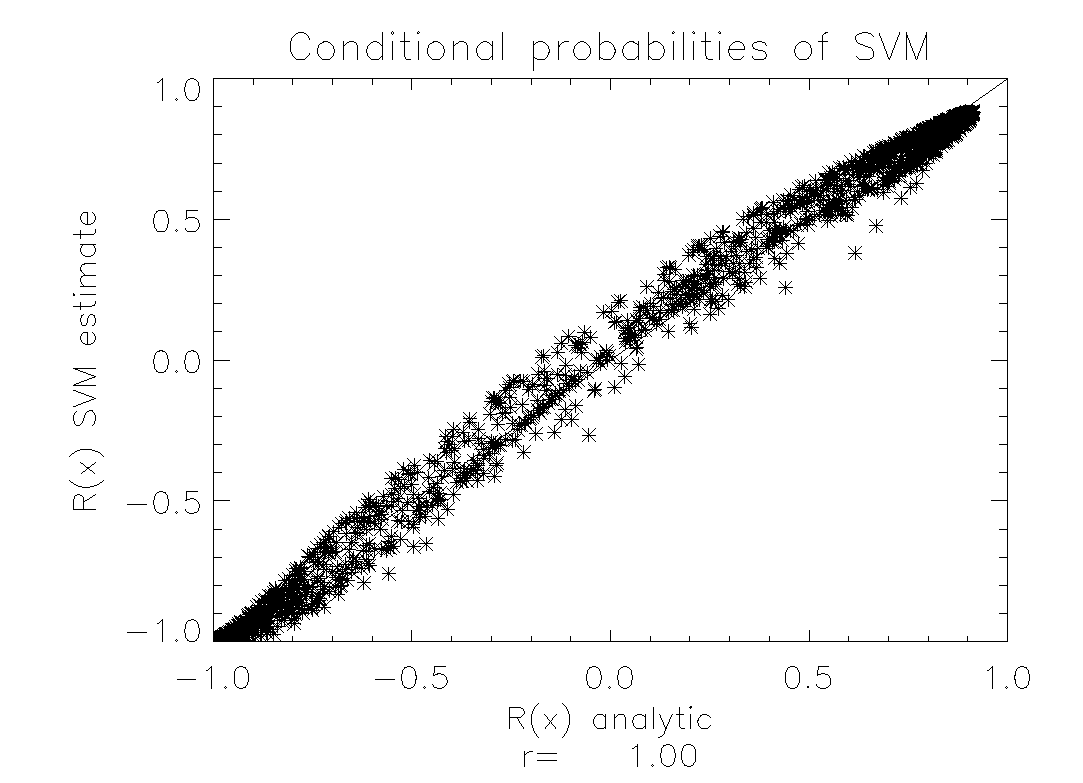
\includegraphics{con_svm.eps}}
%  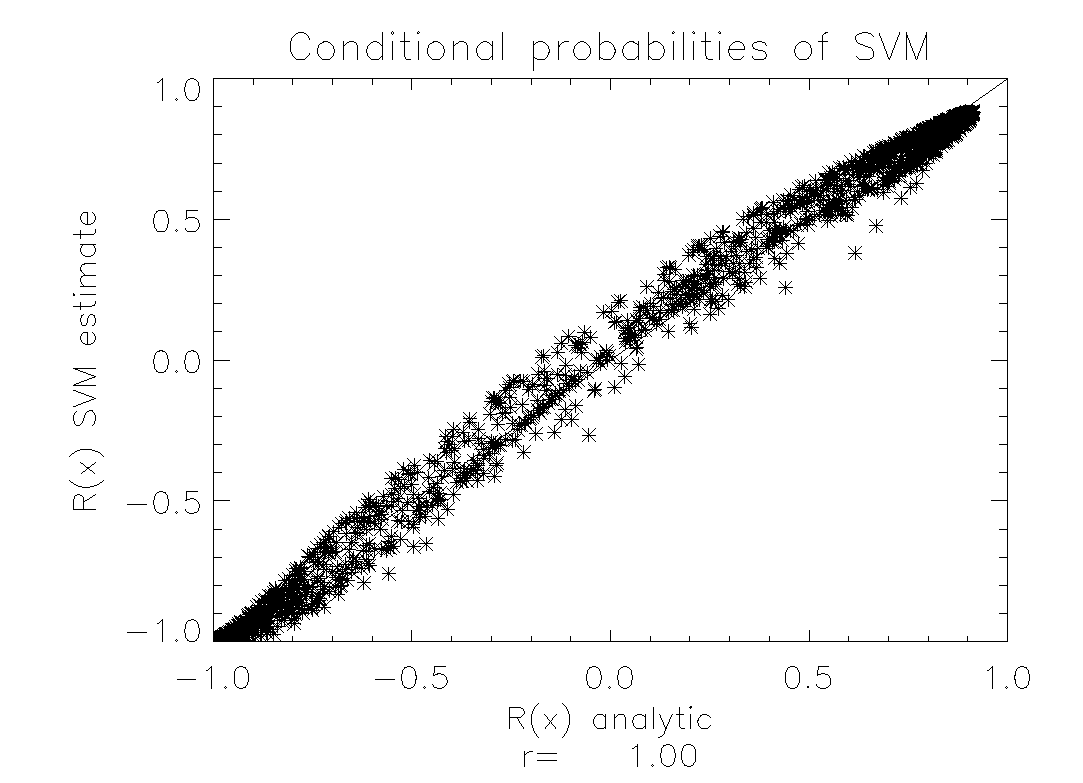
\includegraphics[width=0.9\textwidth]{con_svm.eps}
  \caption{Estimates of conditional probabilities.}
  \label{con_svm}
\end{figure}

\begin{figure}
  \resizebox{0.9\textwidth}{!}{
    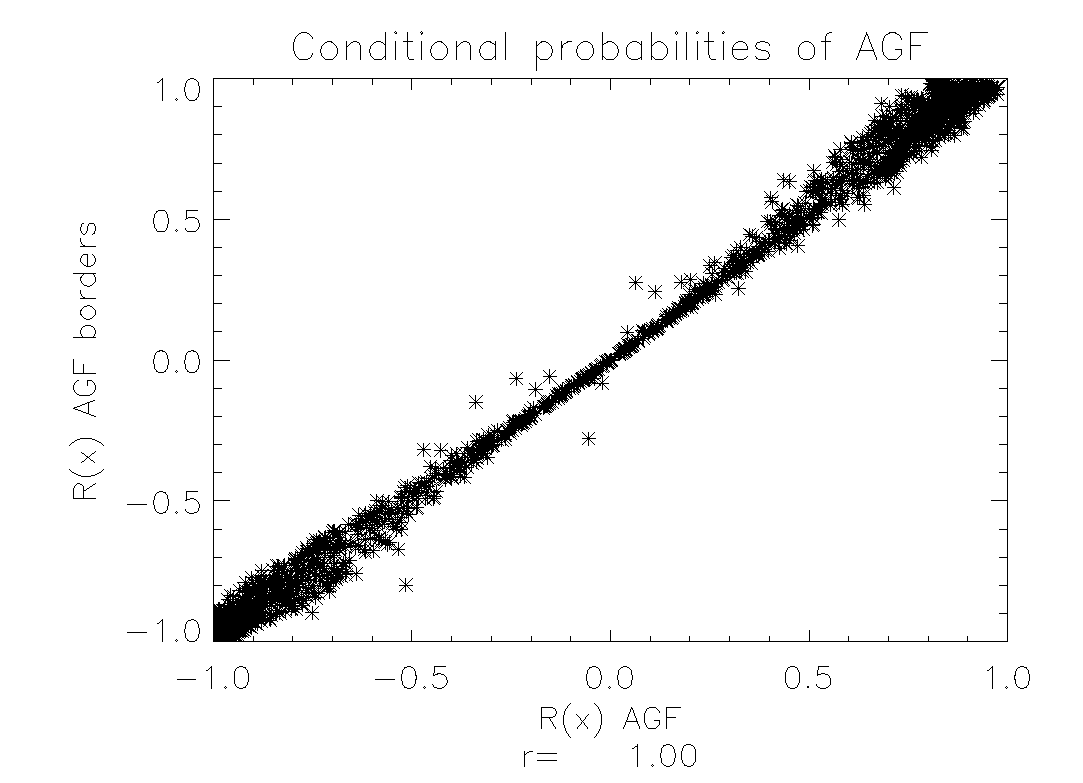
\includegraphics{con_agf2.eps}}
%  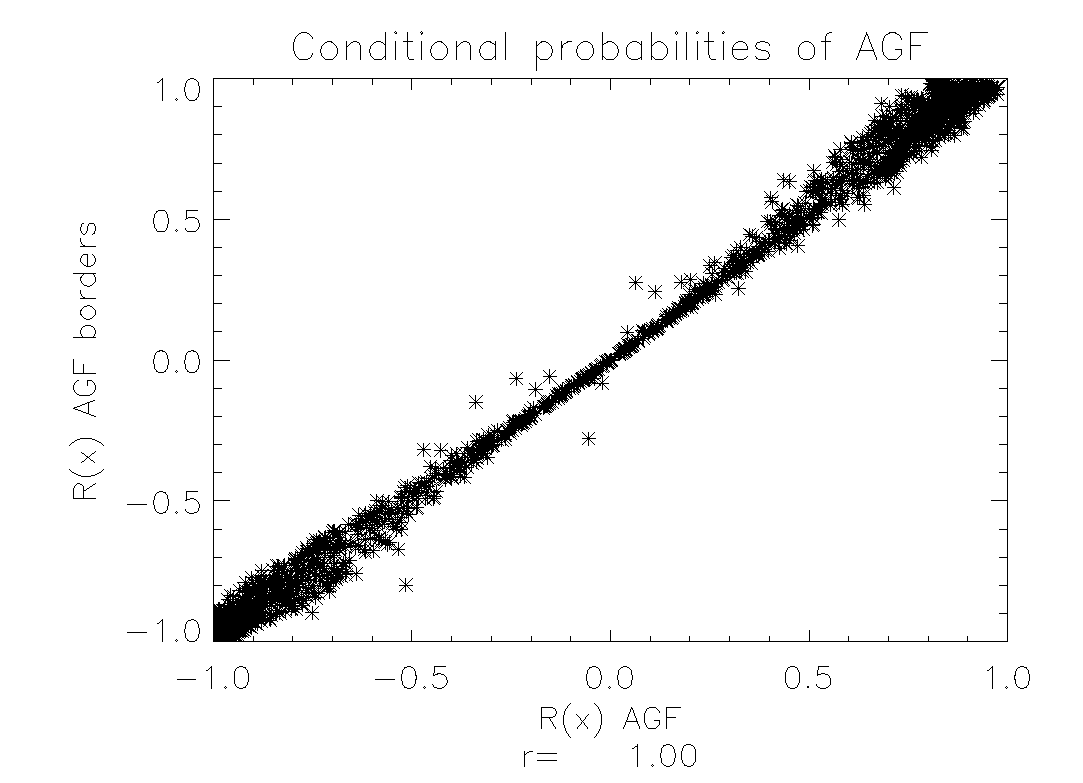
\includegraphics[width=0.9\textwidth]{con_agf2.eps}
  \caption{Estimates of conditional probabilities.}
  \label{con_agf2}
\end{figure}

\section{Discussion}

\begin{figure}
  \resizebox{0.95\textwidth}{!}{
    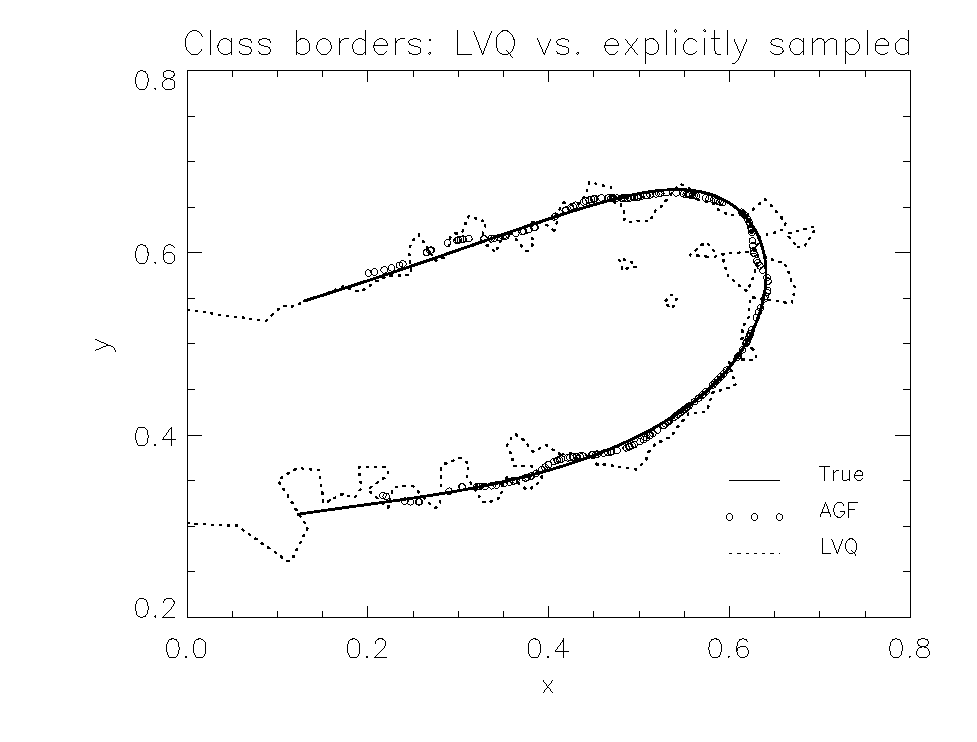
\includegraphics{lvq_vs_brd2.eps}}
%  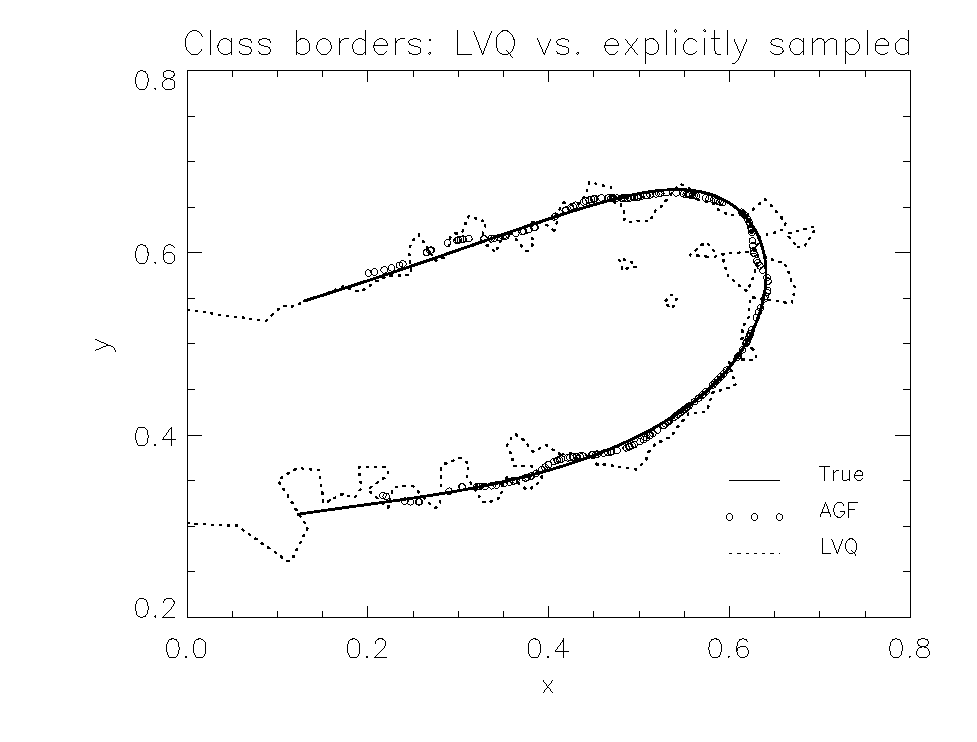
\includegraphics[angle=90, width=0.9\textwidth]{lvq_vs_brd2.ps}
  \label{lvq_vs_brd}
  \caption{The class border}
\end{figure}

When compared with the three other classification methods,
arguably the three most popular available, adaptive
Guassian filtering shows significant advantages in one or
more areas, while possessing few, if any of the other methods'
disadvantages.  
Accuracies of all the methods are identical and approach the Bayesian
limits, except for LVQ.
This is expected for this type of problem and
we are more interested here in differences in speed and in
particular, the accuracies of the conditional probabilities.
The only method that suffers in accuracy is LVQ, despite
the large number of codebook vectors and training cycles.

Learning vector quantization is fast:  training times can
be as little as one (1) second.
Unfortunately, it does not supply any knowledge of the
conditional probabilities, a necessary quantity for measuring
the accuracy of a given classification with no prior knowledge
of its true value.

Another short-coming of the LVQ method is that it samples very
sparsely near the class borders, the exact region where we
require the most knowledge.  In fact the density of codebook
vectors approaches zero at the class border--the method is
actually designed this way!  When we plot the class border
between the codebook vectors from an LVQ training run, this
produces a line that is jagged and meandering.  Contrast this
to the border found via AGF as shown in figure \ref{lvq_vs_brd}.

The main disadvantages of the Support Vector Machine are its slowness
and complexity.  While Adaptive Guassian Filtering has none of
its mathematical sophistication, in fact
I would argue it has all the subtlety of a sledgehammer,
this need not be a point against it.  When generating
numerical estimates of a quantity, why use anything but a
brute-force numerical algorithm?

The slow training time
of the SVM is actually more optimistic than it at first 
appears.  There are so many parameters to select
when applying it and choosing the wrong ones will
frequently result either in nonsense or in the method
failing to converge.  Indeed, the authors of the LIBSVM
go so far as to recommend a grid-search to find the best parameters
of $\gamma$ and $C$. \cite{LIBSVM_guide}

Border training using AGF requires five
parameters, although in principle, it is chiefly
the objective total weight, $W_c$, that the user should
be concerned with.  
The number of nearest neighbours required for the estimate
is closely related--
typically this will be one or two orders of magnitude
larger, although it is difficult to 
reliably approximate the relationship.
Values for $W_c$
of between $25$ and $50$ usually produce good results
but the parameter may best be thought of as a smoothing
coefficient that prevents over-training, much like the
cost term added to the minimization 
procedure of the SVM. \cite{Mueller_etal2001}

For the initial filter width, the total variance of the
data is typically a good choice, although sometimes a
larger value may be required.
The other two parameters, the number of border samples and
the tolerance of border estimates, are easy to select.

Another issue with the SVM is the slow classification time.
This is likely due to inefficient programming since the classification
times of all three methods with an explicit training phase
should be of roughly the same order.

Finally, the conditional probabilities of all methods that return them 
are equally accurate, at least by the numbers, although
the scatter plots might give a better indication.
Likely the AGF borders technique
would not be so accurate for problems that are not so well
conditioned.  This may also be the case for SVM since it works in a 
similar fashion--by fitting to a single-parameter function.
\cite{CC01a}  
More accurate estimates can always be obtained by applying one of the
more direct methods--KNN or AGF without borders training.

Another issue with the conditional probabilities for the
AGF borders is that they are less accurate as their magnitudes
approach one, as can be seen from figures \ref{con_agf_bord} and 
\ref{con_agf2}.  The SVM estimates have the opposite
problem and from the plots appear to be the better-behaved of the
two, although there appears to be a slight bias for low values,
indicating that the borders may be consistently mis-placed.

\section{Conclusion}

A simple classification algorithm was described and validated on a
pair of two-dimensional synthetic test classes.  
It was compared to three other popular
methods:  $k$-nearest-neighbours, learning vector quantization and
support vector machines, as well as the theoretical Bayesian probability
estimates.  As applied to the test case,
it was found to have significant advantages over all three
methods, while possessing few, if any, of their disadvantages.
In its simplicity lies its power:  it is fast, accurate, easy to use
and understand as well as robust.

Further work and improvements to the method would lie on several fronts.  
One would involve adding an error estimate to the
probability estimates.  This could potentially be used to derive
an optimal filter function, as well as add a more rigorous
mathematical justification for the technique, another desired area
for improvement.

Adding some sort of binning for the training samples could improve
the speed further.  To do this with large-dimensional data
sets is tricky, especially when selecting a number of nearest
neighbours instead of all neighbours within a certain radius, but
could potentially increase the time of estimating $R$ for one test point
from of order $n \log k$ to order roughly $\sim k \log n$.  
The undesirable side-effect is an increase in the number of parameters
that need to be tuned.

Border sampling could be improved in a number of ways.  The most
obvious is to even out the distance between the samples.
Existing border samples could be refined using an iterative procedure
that causes nearby samples to be mutually repelled and distant
samples to be attracted, preferably in proportion to the sample
density, while constraining motion to the class
border.

The method could also be tested on some more real-world problems.
Current tests on one (for which it was designed,
in fact) involving discrete
retrieval of water-vapour from satellite data 
show it to be even more advantageous than this
simple validation exercise would suggest.  Preliminary trials
 on other real world problems are equally favourable.

Finally, the method can be generalized for more than two
classes.  This is actually quite trivial and involves
sub-dividing the class types until we need only train for
two classes at a time.  As the number of classes increases,
the number of possible ways of doing this grows 
rapidly to a very large number.



\section*{Acknowledgements}
Thank you very much to my colleaques from the IUP, University of
Bremen for their continued support and encouragement of this work,
in particular Stefan Buehler, Georg Heygster and Oliver Lemke.  
Thanks to Christian Melsheimer for his very valued comments on the first draft.
Thanks especially to the former PEP (Postgraduate program in
Environmental Physics) team, Stefanie Buehler, Prof. Jörn
Bleck-Neuhaus, Christine Schiwek and Barbara Kosak, without whom
I would not have been able to complete my master's degree, from
which this paper is derived.

\bibliography{../agf_bib}

\end{flushleft}
\end{document}

